\documentclass[12pt,a4paper,titlepage]{scrartcl}

\usepackage{comment}
\usepackage[main=ngerman,english]{babel}
\usepackage[utf8]{inputenc}
\usepackage[T1]{fontenc}
\usepackage{lmodern}
\usepackage{geometry}
\geometry{left=2.5cm,right=2.5cm,top=2.5cm,bottom=3cm,head=29pt,foot=25pt}
\setlength{\footheight}{25pt}
\usepackage{microtype}
\usepackage{amsmath,amssymb,mathtools}
\numberwithin{equation}{section}
\numberwithin{table}{section}
\numberwithin{figure}{section}
\usepackage{siunitx}
\sisetup{locale=US, separate-uncertainty=true, per-mode=fraction}
\usepackage{booktabs}
\usepackage{multirow}
\usepackage{graphicx}
\usepackage{float}
\usepackage{caption}
\usepackage{subcaption}
\usepackage[automark]{scrlayer-scrpage}
\usepackage[most]{tcolorbox}
\usepackage{hyperref}
\usepackage{pdfpages}
\usepackage{csvsimple-l3}
\usepackage{longtable}
\usepackage{graphicx}


%
% Basic figure setup, for now with no caption control since it's done
% automatically by Pandoc (which extracts ![](path) syntax from Markdown).
\usepackage{graphicx}
% Keep aspect ratio if custom image width or height is specified
\setkeys{Gin}{keepaspectratio}
% Maintain compatibility with old templates. Remove in nbconvert 6.0
\let\Oldincludegraphics\includegraphics
\usepackage{caption}

\usepackage{float}

\floatplacement{figure}{H} % forces figures to be placed at the correct location
\usepackage{xcolor} % Allow colors to be defined
\usepackage{enumerate} % Needed for markdown enumerations to work
\usepackage{geometry} % Used to adjust the document margins
\usepackage{amsmath} % Equations
\usepackage{amssymb} % Equations
\usepackage{textcomp} % defines textquotesingle
% Hack from http://tex.stackexchange.com/a/47451/13684:
\AtBeginDocument{%
    \def\PYZsq{\textquotesingle}% Upright quotes in Pygmentized code
}
\usepackage{upquote} % Upright quotes for verbatim code
\usepackage{eurosym} % defines \euro

\usepackage{iftex}
\ifPDFTeX
    \usepackage[T1]{fontenc}
    \IfFileExists{alphabeta.sty}{
            \usepackage{alphabeta}
        }{
            \usepackage[mathletters]{ucs}
            \usepackage[utf8x]{inputenc}
        }
\else
    \usepackage{fontspec}
    \usepackage{unicode-math}
\fi

\usepackage{fancyvrb} % verbatim replacement that allows latex
\usepackage{grffile} % extends the file name processing of package graphics
                        % to support a larger range
\makeatletter % fix for old versions of grffile with XeLaTeX
\@ifpackagelater{grffile}{2019/11/01}
{
    % Do nothing on new versions
}
{
    \def\Gread@@xetex#1{%
    \IfFileExists{"\Gin@base".bb}%
    {\Gread@eps{\Gin@base.bb}}%
    {\Gread@@xetex@aux#1}%
    }
}
\makeatother
\usepackage[Export]{adjustbox} % Used to constrain images to a maximum size
\adjustboxset{max size={0.9\linewidth}{0.9\paperheight}}

% The hyperref package gives us a pdf with properly built
% internal navigation ('pdf bookmarks' for the table of contents,
% internal cross-reference links, web links for URLs, etc.)
\usepackage{hyperref}
% The default LaTeX title has an obnoxious amount of whitespace. By default,
% titling removes some of it. It also provides customization options.
\usepackage{titling}
\usepackage{longtable} % longtable support required by pandoc >1.10
\usepackage{booktabs}  % table support for pandoc > 1.12.2
\usepackage{array}     % table support for pandoc >= 2.11.3
\usepackage{calc}      % table minipage width calculation for pandoc >= 2.11.1
\usepackage[inline]{enumitem} % IRkernel/repr support (it uses the enumerate* environment)
\usepackage[normalem]{ulem} % ulem is needed to support strikethroughs (\sout)
                            % normalem makes italics be italics, not underlines
\usepackage{soul}      % strikethrough (\st) support for pandoc >= 3.0.0
\usepackage{mathrsfs}



% Colors for the hyperref package
\definecolor{urlcolor}{rgb}{0,.145,.698}
\definecolor{linkcolor}{rgb}{.71,0.21,0.01}
\definecolor{citecolor}{rgb}{.12,.54,.11}

% ANSI colors
\definecolor{ansi-black}{HTML}{3E424D}
\definecolor{ansi-black-intense}{HTML}{282C36}
\definecolor{ansi-red}{HTML}{E75C58}
\definecolor{ansi-red-intense}{HTML}{B22B31}
\definecolor{ansi-green}{HTML}{00A250}
\definecolor{ansi-green-intense}{HTML}{007427}
\definecolor{ansi-yellow}{HTML}{DDB62B}
\definecolor{ansi-yellow-intense}{HTML}{B27D12}
\definecolor{ansi-blue}{HTML}{208FFB}
\definecolor{ansi-blue-intense}{HTML}{0065CA}
\definecolor{ansi-magenta}{HTML}{D160C4}
\definecolor{ansi-magenta-intense}{HTML}{A03196}
\definecolor{ansi-cyan}{HTML}{60C6C8}
\definecolor{ansi-cyan-intense}{HTML}{258F8F}
\definecolor{ansi-white}{HTML}{C5C1B4}
\definecolor{ansi-white-intense}{HTML}{A1A6B2}
\definecolor{ansi-default-inverse-fg}{HTML}{FFFFFF}
\definecolor{ansi-default-inverse-bg}{HTML}{000000}

% common color for the border for error outputs.
\definecolor{outerrorbackground}{HTML}{FFDFDF}

% commands and environments needed by pandoc snippets
% extracted from the output of `pandoc -s`
\providecommand{\tightlist}{%
    \setlength{\itemsep}{0pt}\setlength{\parskip}{0pt}}
\DefineVerbatimEnvironment{Highlighting}{Verbatim}{commandchars=\\\{\}}
% Add ',fontsize=\small' for more characters per line
\newenvironment{Shaded}{}{}
\newcommand{\KeywordTok}[1]{\textcolor[rgb]{0.00,0.44,0.13}{\textbf{{#1}}}}
\newcommand{\DataTypeTok}[1]{\textcolor[rgb]{0.56,0.13,0.00}{{#1}}}
\newcommand{\DecValTok}[1]{\textcolor[rgb]{0.25,0.63,0.44}{{#1}}}
\newcommand{\BaseNTok}[1]{\textcolor[rgb]{0.25,0.63,0.44}{{#1}}}
\newcommand{\FloatTok}[1]{\textcolor[rgb]{0.25,0.63,0.44}{{#1}}}
\newcommand{\CharTok}[1]{\textcolor[rgb]{0.25,0.44,0.63}{{#1}}}
\newcommand{\StringTok}[1]{\textcolor[rgb]{0.25,0.44,0.63}{{#1}}}
\newcommand{\CommentTok}[1]{\textcolor[rgb]{0.38,0.63,0.69}{\textit{{#1}}}}
\newcommand{\OtherTok}[1]{\textcolor[rgb]{0.00,0.44,0.13}{{#1}}}
\newcommand{\AlertTok}[1]{\textcolor[rgb]{1.00,0.00,0.00}{\textbf{{#1}}}}
\newcommand{\FunctionTok}[1]{\textcolor[rgb]{0.02,0.16,0.49}{{#1}}}
\newcommand{\RegionMarkerTok}[1]{{#1}}
\newcommand{\ErrorTok}[1]{\textcolor[rgb]{1.00,0.00,0.00}{\textbf{{#1}}}}
\newcommand{\NormalTok}[1]{{#1}}

% Additional commands for more recent versions of Pandoc
\newcommand{\ConstantTok}[1]{\textcolor[rgb]{0.53,0.00,0.00}{{#1}}}
\newcommand{\SpecialCharTok}[1]{\textcolor[rgb]{0.25,0.44,0.63}{{#1}}}
\newcommand{\VerbatimStringTok}[1]{\textcolor[rgb]{0.25,0.44,0.63}{{#1}}}
\newcommand{\SpecialStringTok}[1]{\textcolor[rgb]{0.73,0.40,0.53}{{#1}}}
\newcommand{\ImportTok}[1]{{#1}}
\newcommand{\DocumentationTok}[1]{\textcolor[rgb]{0.73,0.13,0.13}{\textit{{#1}}}}
\newcommand{\AnnotationTok}[1]{\textcolor[rgb]{0.38,0.63,0.69}{\textbf{\textit{{#1}}}}}
\newcommand{\CommentVarTok}[1]{\textcolor[rgb]{0.38,0.63,0.69}{\textbf{\textit{{#1}}}}}
\newcommand{\VariableTok}[1]{\textcolor[rgb]{0.10,0.09,0.49}{{#1}}}
\newcommand{\ControlFlowTok}[1]{\textcolor[rgb]{0.00,0.44,0.13}{\textbf{{#1}}}}
\newcommand{\OperatorTok}[1]{\textcolor[rgb]{0.40,0.40,0.40}{{#1}}}
\newcommand{\BuiltInTok}[1]{{#1}}
\newcommand{\ExtensionTok}[1]{{#1}}
\newcommand{\PreprocessorTok}[1]{\textcolor[rgb]{0.74,0.48,0.00}{{#1}}}
\newcommand{\AttributeTok}[1]{\textcolor[rgb]{0.49,0.56,0.16}{{#1}}}
\newcommand{\InformationTok}[1]{\textcolor[rgb]{0.38,0.63,0.69}{\textbf{\textit{{#1}}}}}
\newcommand{\WarningTok}[1]{\textcolor[rgb]{0.38,0.63,0.69}{\textbf{\textit{{#1}}}}}
\makeatletter
\newsavebox\pandoc@box
\newcommand*\pandocbounded[1]{%
    \sbox\pandoc@box{#1}%
    % scaling factors for width and height
    \Gscale@div\@tempa\textheight{\dimexpr\ht\pandoc@box+\dp\pandoc@box\relax}%
    \Gscale@div\@tempb\linewidth{\wd\pandoc@box}%
    % select the smaller of both
    \ifdim\@tempb\p@<\@tempa\p@
    \let\@tempa\@tempb
    \fi
    % scaling accordingly (\@tempa < 1)
    \ifdim\@tempa\p@<\p@
    \scalebox{\@tempa}{\usebox\pandoc@box}%
    % scaling not needed, use as it is
    \else
    \usebox{\pandoc@box}%
    \fi
}
\makeatother

% Define a nice break command that doesn't care if a line doesn't already
% exist.
\def\br{\hspace*{\fill} \\* }
% Math Jax compatibility definitions
\def\gt{>}
\def\lt{<}
\let\Oldtex\TeX
\let\Oldlatex\LaTeX
\renewcommand{\TeX}{\textrm{\Oldtex}}
\renewcommand{\LaTeX}{\textrm{\Oldlatex}}
% Document parameters
% Document title
\title{U-I-Diagramm}
    

    
    
    
    
    
% Pygments definitions
\makeatletter
\def\PY@reset{\let\PY@it=\relax \let\PY@bf=\relax%
    \let\PY@ul=\relax \let\PY@tc=\relax%
    \let\PY@bc=\relax \let\PY@ff=\relax}
\def\PY@tok#1{\csname PY@tok@#1\endcsname}
\def\PY@toks#1+{\ifx\relax#1\empty\else%
    \PY@tok{#1}\expandafter\PY@toks\fi}
\def\PY@do#1{\PY@bc{\PY@tc{\PY@ul{%
    \PY@it{\PY@bf{\PY@ff{#1}}}}}}}
\def\PY#1#2{\PY@reset\PY@toks#1+\relax+\PY@do{#2}}

\@namedef{PY@tok@w}{\def\PY@tc##1{\textcolor[rgb]{0.73,0.73,0.73}{##1}}}
\@namedef{PY@tok@c}{\let\PY@it=\textit\def\PY@tc##1{\textcolor[rgb]{0.24,0.48,0.48}{##1}}}
\@namedef{PY@tok@cp}{\def\PY@tc##1{\textcolor[rgb]{0.61,0.40,0.00}{##1}}}
\@namedef{PY@tok@k}{\let\PY@bf=\textbf\def\PY@tc##1{\textcolor[rgb]{0.00,0.50,0.00}{##1}}}
\@namedef{PY@tok@kp}{\def\PY@tc##1{\textcolor[rgb]{0.00,0.50,0.00}{##1}}}
\@namedef{PY@tok@kt}{\def\PY@tc##1{\textcolor[rgb]{0.69,0.00,0.25}{##1}}}
\@namedef{PY@tok@o}{\def\PY@tc##1{\textcolor[rgb]{0.40,0.40,0.40}{##1}}}
\@namedef{PY@tok@ow}{\let\PY@bf=\textbf\def\PY@tc##1{\textcolor[rgb]{0.67,0.13,1.00}{##1}}}
\@namedef{PY@tok@nb}{\def\PY@tc##1{\textcolor[rgb]{0.00,0.50,0.00}{##1}}}
\@namedef{PY@tok@nf}{\def\PY@tc##1{\textcolor[rgb]{0.00,0.00,1.00}{##1}}}
\@namedef{PY@tok@nc}{\let\PY@bf=\textbf\def\PY@tc##1{\textcolor[rgb]{0.00,0.00,1.00}{##1}}}
\@namedef{PY@tok@nn}{\let\PY@bf=\textbf\def\PY@tc##1{\textcolor[rgb]{0.00,0.00,1.00}{##1}}}
\@namedef{PY@tok@ne}{\let\PY@bf=\textbf\def\PY@tc##1{\textcolor[rgb]{0.80,0.25,0.22}{##1}}}
\@namedef{PY@tok@nv}{\def\PY@tc##1{\textcolor[rgb]{0.10,0.09,0.49}{##1}}}
\@namedef{PY@tok@no}{\def\PY@tc##1{\textcolor[rgb]{0.53,0.00,0.00}{##1}}}
\@namedef{PY@tok@nl}{\def\PY@tc##1{\textcolor[rgb]{0.46,0.46,0.00}{##1}}}
\@namedef{PY@tok@ni}{\let\PY@bf=\textbf\def\PY@tc##1{\textcolor[rgb]{0.44,0.44,0.44}{##1}}}
\@namedef{PY@tok@na}{\def\PY@tc##1{\textcolor[rgb]{0.41,0.47,0.13}{##1}}}
\@namedef{PY@tok@nt}{\let\PY@bf=\textbf\def\PY@tc##1{\textcolor[rgb]{0.00,0.50,0.00}{##1}}}
\@namedef{PY@tok@nd}{\def\PY@tc##1{\textcolor[rgb]{0.67,0.13,1.00}{##1}}}
\@namedef{PY@tok@s}{\def\PY@tc##1{\textcolor[rgb]{0.73,0.13,0.13}{##1}}}
\@namedef{PY@tok@sd}{\let\PY@it=\textit\def\PY@tc##1{\textcolor[rgb]{0.73,0.13,0.13}{##1}}}
\@namedef{PY@tok@si}{\let\PY@bf=\textbf\def\PY@tc##1{\textcolor[rgb]{0.64,0.35,0.47}{##1}}}
\@namedef{PY@tok@se}{\let\PY@bf=\textbf\def\PY@tc##1{\textcolor[rgb]{0.67,0.36,0.12}{##1}}}
\@namedef{PY@tok@sr}{\def\PY@tc##1{\textcolor[rgb]{0.64,0.35,0.47}{##1}}}
\@namedef{PY@tok@ss}{\def\PY@tc##1{\textcolor[rgb]{0.10,0.09,0.49}{##1}}}
\@namedef{PY@tok@sx}{\def\PY@tc##1{\textcolor[rgb]{0.00,0.50,0.00}{##1}}}
\@namedef{PY@tok@m}{\def\PY@tc##1{\textcolor[rgb]{0.40,0.40,0.40}{##1}}}
\@namedef{PY@tok@gh}{\let\PY@bf=\textbf\def\PY@tc##1{\textcolor[rgb]{0.00,0.00,0.50}{##1}}}
\@namedef{PY@tok@gu}{\let\PY@bf=\textbf\def\PY@tc##1{\textcolor[rgb]{0.50,0.00,0.50}{##1}}}
\@namedef{PY@tok@gd}{\def\PY@tc##1{\textcolor[rgb]{0.63,0.00,0.00}{##1}}}
\@namedef{PY@tok@gi}{\def\PY@tc##1{\textcolor[rgb]{0.00,0.52,0.00}{##1}}}
\@namedef{PY@tok@gr}{\def\PY@tc##1{\textcolor[rgb]{0.89,0.00,0.00}{##1}}}
\@namedef{PY@tok@ge}{\let\PY@it=\textit}
\@namedef{PY@tok@gs}{\let\PY@bf=\textbf}
\@namedef{PY@tok@ges}{\let\PY@bf=\textbf\let\PY@it=\textit}
\@namedef{PY@tok@gp}{\let\PY@bf=\textbf\def\PY@tc##1{\textcolor[rgb]{0.00,0.00,0.50}{##1}}}
\@namedef{PY@tok@go}{\def\PY@tc##1{\textcolor[rgb]{0.44,0.44,0.44}{##1}}}
\@namedef{PY@tok@gt}{\def\PY@tc##1{\textcolor[rgb]{0.00,0.27,0.87}{##1}}}
\@namedef{PY@tok@err}{\def\PY@bc##1{{\setlength{\fboxsep}{\string -\fboxrule}\fcolorbox[rgb]{1.00,0.00,0.00}{1,1,1}{\strut ##1}}}}
\@namedef{PY@tok@kc}{\let\PY@bf=\textbf\def\PY@tc##1{\textcolor[rgb]{0.00,0.50,0.00}{##1}}}
\@namedef{PY@tok@kd}{\let\PY@bf=\textbf\def\PY@tc##1{\textcolor[rgb]{0.00,0.50,0.00}{##1}}}
\@namedef{PY@tok@kn}{\let\PY@bf=\textbf\def\PY@tc##1{\textcolor[rgb]{0.00,0.50,0.00}{##1}}}
\@namedef{PY@tok@kr}{\let\PY@bf=\textbf\def\PY@tc##1{\textcolor[rgb]{0.00,0.50,0.00}{##1}}}
\@namedef{PY@tok@bp}{\def\PY@tc##1{\textcolor[rgb]{0.00,0.50,0.00}{##1}}}
\@namedef{PY@tok@fm}{\def\PY@tc##1{\textcolor[rgb]{0.00,0.00,1.00}{##1}}}
\@namedef{PY@tok@vc}{\def\PY@tc##1{\textcolor[rgb]{0.10,0.09,0.49}{##1}}}
\@namedef{PY@tok@vg}{\def\PY@tc##1{\textcolor[rgb]{0.10,0.09,0.49}{##1}}}
\@namedef{PY@tok@vi}{\def\PY@tc##1{\textcolor[rgb]{0.10,0.09,0.49}{##1}}}
\@namedef{PY@tok@vm}{\def\PY@tc##1{\textcolor[rgb]{0.10,0.09,0.49}{##1}}}
\@namedef{PY@tok@sa}{\def\PY@tc##1{\textcolor[rgb]{0.73,0.13,0.13}{##1}}}
\@namedef{PY@tok@sb}{\def\PY@tc##1{\textcolor[rgb]{0.73,0.13,0.13}{##1}}}
\@namedef{PY@tok@sc}{\def\PY@tc##1{\textcolor[rgb]{0.73,0.13,0.13}{##1}}}
\@namedef{PY@tok@dl}{\def\PY@tc##1{\textcolor[rgb]{0.73,0.13,0.13}{##1}}}
\@namedef{PY@tok@s2}{\def\PY@tc##1{\textcolor[rgb]{0.73,0.13,0.13}{##1}}}
\@namedef{PY@tok@sh}{\def\PY@tc##1{\textcolor[rgb]{0.73,0.13,0.13}{##1}}}
\@namedef{PY@tok@s1}{\def\PY@tc##1{\textcolor[rgb]{0.73,0.13,0.13}{##1}}}
\@namedef{PY@tok@mb}{\def\PY@tc##1{\textcolor[rgb]{0.40,0.40,0.40}{##1}}}
\@namedef{PY@tok@mf}{\def\PY@tc##1{\textcolor[rgb]{0.40,0.40,0.40}{##1}}}
\@namedef{PY@tok@mh}{\def\PY@tc##1{\textcolor[rgb]{0.40,0.40,0.40}{##1}}}
\@namedef{PY@tok@mi}{\def\PY@tc##1{\textcolor[rgb]{0.40,0.40,0.40}{##1}}}
\@namedef{PY@tok@il}{\def\PY@tc##1{\textcolor[rgb]{0.40,0.40,0.40}{##1}}}
\@namedef{PY@tok@mo}{\def\PY@tc##1{\textcolor[rgb]{0.40,0.40,0.40}{##1}}}
\@namedef{PY@tok@ch}{\let\PY@it=\textit\def\PY@tc##1{\textcolor[rgb]{0.24,0.48,0.48}{##1}}}
\@namedef{PY@tok@cm}{\let\PY@it=\textit\def\PY@tc##1{\textcolor[rgb]{0.24,0.48,0.48}{##1}}}
\@namedef{PY@tok@cpf}{\let\PY@it=\textit\def\PY@tc##1{\textcolor[rgb]{0.24,0.48,0.48}{##1}}}
\@namedef{PY@tok@c1}{\let\PY@it=\textit\def\PY@tc##1{\textcolor[rgb]{0.24,0.48,0.48}{##1}}}
\@namedef{PY@tok@cs}{\let\PY@it=\textit\def\PY@tc##1{\textcolor[rgb]{0.24,0.48,0.48}{##1}}}

\def\PYZbs{\char`\\}
\def\PYZus{\char`\_}
\def\PYZob{\char`\{}
\def\PYZcb{\char`\}}
\def\PYZca{\char`\^}
\def\PYZam{\char`\&}
\def\PYZlt{\char`\<}
\def\PYZgt{\char`\>}
\def\PYZsh{\char`\#}
\def\PYZpc{\char`\%}
\def\PYZdl{\char`\$}
\def\PYZhy{\char`\-}
\def\PYZsq{\char`\'}
\def\PYZdq{\char`\"}
\def\PYZti{\char`\~}
% for compatibility with earlier versions
\def\PYZat{@}
\def\PYZlb{[}
\def\PYZrb{]}
\makeatother


    % For linebreaks inside Verbatim environment from package fancyvrb.
    \makeatletter
        \newbox\Wrappedcontinuationbox
        \newbox\Wrappedvisiblespacebox
        \newcommand*\Wrappedvisiblespace {\textcolor{red}{\textvisiblespace}}
        \newcommand*\Wrappedcontinuationsymbol {\textcolor{red}{\llap{\tiny$\m@th\hookrightarrow$}}}
        \newcommand*\Wrappedcontinuationindent {3ex }
        \newcommand*\Wrappedafterbreak {\kern\Wrappedcontinuationindent\copy\Wrappedcontinuationbox}
        % Take advantage of the already applied Pygments mark-up to insert
        % potential linebreaks for TeX processing.
        %        {, <, #, %, $, ' and ": go to next line.
        %        _, }, ^, &, >, - and ~: stay at end of broken line.
        % Use of \textquotesingle for straight quote.
        \newcommand*\Wrappedbreaksatspecials {%
            \def\PYGZus{\discretionary{\char`\_}{\Wrappedafterbreak}{\char`\_}}%
            \def\PYGZob{\discretionary{}{\Wrappedafterbreak\char`\{}{\char`\{}}%
            \def\PYGZcb{\discretionary{\char`\}}{\Wrappedafterbreak}{\char`\}}}%
            \def\PYGZca{\discretionary{\char`\^}{\Wrappedafterbreak}{\char`\^}}%
            \def\PYGZam{\discretionary{\char`\&}{\Wrappedafterbreak}{\char`\&}}%
            \def\PYGZlt{\discretionary{}{\Wrappedafterbreak\char`\<}{\char`\<}}%
            \def\PYGZgt{\discretionary{\char`\>}{\Wrappedafterbreak}{\char`\>}}%
            \def\PYGZsh{\discretionary{}{\Wrappedafterbreak\char`\#}{\char`\#}}%
            \def\PYGZpc{\discretionary{}{\Wrappedafterbreak\char`\%}{\char`\%}}%
            \def\PYGZdl{\discretionary{}{\Wrappedafterbreak\char`\$}{\char`\$}}%
            \def\PYGZhy{\discretionary{\char`\-}{\Wrappedafterbreak}{\char`\-}}%
            \def\PYGZsq{\discretionary{}{\Wrappedafterbreak\textquotesingle}{\textquotesingle}}%
            \def\PYGZdq{\discretionary{}{\Wrappedafterbreak\char`\"}{\char`\"}}%
            \def\PYGZti{\discretionary{\char`\~}{\Wrappedafterbreak}{\char`\~}}%
        }
        % Some characters . , ; ? ! / are not pygmentized.
        % This macro makes them "active" and they will insert potential linebreaks
        \newcommand*\Wrappedbreaksatpunct {%
            \lccode`\~`\.\lowercase{\def~}{\discretionary{\hbox{\char`\.}}{\Wrappedafterbreak}{\hbox{\char`\.}}}%
            \lccode`\~`\,\lowercase{\def~}{\discretionary{\hbox{\char`\,}}{\Wrappedafterbreak}{\hbox{\char`\,}}}%
            \lccode`\~`\;\lowercase{\def~}{\discretionary{\hbox{\char`\;}}{\Wrappedafterbreak}{\hbox{\char`\;}}}%
            \lccode`\~`\:\lowercase{\def~}{\discretionary{\hbox{\char`\:}}{\Wrappedafterbreak}{\hbox{\char`\:}}}%
            \lccode`\~`\?\lowercase{\def~}{\discretionary{\hbox{\char`\?}}{\Wrappedafterbreak}{\hbox{\char`\?}}}%
            \lccode`\~`\!\lowercase{\def~}{\discretionary{\hbox{\char`\!}}{\Wrappedafterbreak}{\hbox{\char`\!}}}%
            \lccode`\~`\/\lowercase{\def~}{\discretionary{\hbox{\char`\/}}{\Wrappedafterbreak}{\hbox{\char`\/}}}%
            \catcode`\.\active
            \catcode`\,\active
            \catcode`\;\active
            \catcode`\:\active
            \catcode`\?\active
            \catcode`\!\active
            \catcode`\/\active
            \lccode`\~`\~
        }
    \makeatother

    \let\OriginalVerbatim=\Verbatim
    \makeatletter
    \renewcommand{\Verbatim}[1][1]{%
        %\parskip\z@skip
        \sbox\Wrappedcontinuationbox {\Wrappedcontinuationsymbol}%
        \sbox\Wrappedvisiblespacebox {\FV@SetupFont\Wrappedvisiblespace}%
        \def\FancyVerbFormatLine ##1{\hsize\linewidth
            \vtop{\raggedright\hyphenpenalty\z@\exhyphenpenalty\z@
                \doublehyphendemerits\z@\finalhyphendemerits\z@
                \strut ##1\strut}%
        }%
        % If the linebreak is at a space, the latter will be displayed as visible
        % space at end of first line, and a continuation symbol starts next line.
        % Stretch/shrink are however usually zero for typewriter font.
        \def\FV@Space {%
            \nobreak\hskip\z@ plus\fontdimen3\font minus\fontdimen4\font
            \discretionary{\copy\Wrappedvisiblespacebox}{\Wrappedafterbreak}
            {\kern\fontdimen2\font}%
        }%

        % Allow breaks at special characters using \PYG... macros.
        \Wrappedbreaksatspecials
        % Breaks at punctuation characters . , ; ? ! and / need catcode=\active
        \OriginalVerbatim[#1,codes*=\Wrappedbreaksatpunct]%
    }
    \makeatother

    % Exact colors from NB
    \definecolor{incolor}{HTML}{303F9F}
    \definecolor{outcolor}{HTML}{D84315}
    \definecolor{cellborder}{HTML}{CFCFCF}
    \definecolor{cellbackground}{HTML}{F7F7F7}

    % prompt
    \makeatletter
    \newcommand{\boxspacing}{\kern\kvtcb@left@rule\kern\kvtcb@boxsep}
    \makeatother
    \newcommand{\prompt}[4]{
        {\ttfamily\llap{{\color{#2}[#3]:\hspace{3pt}#4}}\vspace{-\baselineskip}}
    }
    

    
    % Prevent overflowing lines due to hard-to-break entities
    \sloppy
    % Setup hyperref package
    \hypersetup{
      breaklinks=true,  % so long urls are correctly broken across lines
      colorlinks=true,
      urlcolor=urlcolor,
      linkcolor=linkcolor,
      citecolor=citecolor,
      }
    % Slightly bigger margins than the latex defaults
    
    \geometry{verbose,tmargin=1in,bmargin=1in,lmargin=1in,rmargin=1in}
    
    


% jupyter nbconvert --to latex 'Path'
% enferne usepackages und begin{document} und end{document}
% \include in main.tex mit \include{Path}


\newcommand{\pdfabbildung}[2]{%
    \refstepcounter{figure}%
    \addcontentsline{lof}{figure}{\protect\numberline{\thefigure}#1}%
    \label{#2}%
}

\newcommand{\pdftabelle}[2]{%
    \refstepcounter{table}%
    \addcontentsline{lot}{table}{\protect\numberline{\thetable}#1}%
    \label{#2}%
}


\hypersetup{colorlinks=true, linkcolor=blue!60!black, urlcolor=blue!60!black, citecolor=blue!60!black}

\clearpairofpagestyles

\chead{%
    \versuch\hfill\autor\\
    \rule{\textwidth}{0.2pt}%
}
\cfoot{%
    \rule{\textwidth}{0.2pt}\\[-0.5ex]
    \pagemark\ 
}
\addtokomafont{pagefoot}{\small}
\setlength{\parindent}{0pt}

\newtcolorbox{resultbox}[1][]{ 
    enhanced,
    colback=black!4!white,
    colframe=black!65!black,
    boxrule=0.8pt,
    arc=0.0mm,
    title=#1,
    fonttitle=\bfseries,
    %drop shadow
}


\newcommand{\versuch}{Versuch 243}
\newcommand{\titel}{Thermisches Rauschen}
\newcommand{\praktikum}{Physikalisches Anfängerpraktikum 2.2}
\newcommand{\autor}{Jonathan Gießen}
\newcommand{\partner}{Sinan Uysal}
\newcommand{\gruppe}{Gruppe 2}
\newcommand{\datum}{28. Oktober 2026}
\newcommand{\betreuer}{Alicia Schneider}

\begin{document}

\pagestyle{scrheadings}

\begin{titlepage}



    \centering
    \vspace*{4cm}
    {\large Universität Heidelberg\par}
    {\small Fakultät für Physik und Astronomie\par}
    {\Large \praktikum\par}
    \vspace{0.8cm}
    {\LARGE \bfseries \versuch\ -- \titel\par}
    \vspace{1.5cm}

    \begin{tabular}{ll}
        \textbf{Autor:} & \autor\\
        \textbf{Partner:} & \partner\\
        \textbf{Gruppe:} & \gruppe\\
        \textbf{Betreuer:} & \betreuer\\
        \textbf{Versuchsdatum:} & \datum\\
    \end{tabular}

    \vfill
    \hrulefill\
\end{titlepage}

\tableofcontents

\bigskip
\begin{tcolorbox}[colback=gray!5,colframe=gray!60,boxrule=0.8pt,arc=0.01mm,title=KI-Hinweis]
    Für die sprachliche Formulierung dieses Protokolls wurde in der Einleitung~\ref{sec:Einleitung} und bei Grundlagen!~\ref{sec:Grundlagen} KI-gestützte Textgenerierung verwendet. 
\end{tcolorbox}.

\clearpage


\section{Einleitung}\label{sec:Einleitung}
Bei einer Temperatur von $T > \SI{0}{\kelvin}$ kommt es in jedem elektrischen Leiter aufgrund der thermischen Anregung zu einer ungeordneten Brownschen Bewegung der freien Ladungsträger. Selbst wenn keine äußere Spannung anliegt, führt diese statistische Bewegung zu kurzzeitigen Ladungsverschiebungen und damit zu einer zeitlich fluktuierenden Spannung an den Enden des Leiters, die als \emph{thermisches Rauschen} bezeichnet wird.

In der praktischen Messtechnik stellt das thermische Rauschen physikalische Grenzen für die Nachweisempfindlichkeit kleiner elektrischer Signale dar, die sich nur durch Kühlung, Mittelwertbildung oder eine Begrenzung der Messbandbreite reduzieren lassen. Jedoch kann sich das Rauschen auch unmittelbar mit der thermischen Energie $k_B T$ zur Temperaturbestimmung zum Beispiel in einem Rauschthermometer zu Nutze gemacht werden.

\medskip
Ziel des vorliegenden Versuchs~243 ist es, das Rauschspektrum ohmscher Widerstände qualitativ zu untersuchen, den Frequenzgang sowie die äquivalente Rauschbandbreite der verwendeten Verstärker- und Filterelektronik zu bestimmen und aus der Abhängigkeit der Rauschspannung vom Widerstandswert bei Raumtemperatur die Boltzmannkonstante $k_B$ zu ermitteln.

\section{Grundlagen und Theorie}\label{sec:Grundlagen}

\subsection{Thermisches Rauschen und Nyquist-Beziehung}
In einem ohmschen Widerstand $R$, der sich im thermischen Gleichgewicht bei der absoluten Temperatur $T$ befindet, führen die Leitungselektronen infolge Stößen mit dem Kristallgitter eine ungerichtete thermische Zufallsbewegung aus. Da keine Raumrichtung bevorzugt ist, verschwindet der zeitliche Mittelwert der resultierenden Rauschspannung $U_r(t)$ an den Klemmen des Widerstands:
\begin{equation}
    \langle U_r \rangle = \lim_{t' \to \infty} \frac{1}{t'} \int_{0}^{t'} U_r(t)\,\mathrm{d}t = 0 \,.
    \label{eq:mittelwert}
\end{equation}
Zur quantitativen Beschreibung der Rauschspannung wird daher ihr Effektivwert $U_{r,\text{eff}} = \sqrt{\langle U_r^2 \rangle}$, also die Wurzel aus dem zeitlichen Mittelwert des Spannungsquadrats, herangezogen:
\begin{equation}
    \sqrt{\langle U_r^2 \rangle} = \sqrt{\lim_{t' \to \infty} \frac{1}{t'} \int_{0}^{t'} U_r^2(t)\,\mathrm{d}t} \,.
    \label{eq:effektivwert}
\end{equation}
Im Frequenzspektrum einer thermischen Rauschquelle sind bis in den Terahertz-Bereich alle Frequenzen mit gleicher Leistungsdichte vertreten, weshalb man wie beim weißen Licht von \emph{weißem Rauschen} spricht. Für das mittlere Spannungsquadrat innerhalb einer Messbandbreite $\Delta f$ gilt die die \emph{Nyquist-Beziehung} \cite{PAPskript}:
\begin{equation}
    \langle U_r^2 \rangle = 4 k_B T R \Delta f \,,
    \label{eq:nyquist}
\end{equation}
wobei $k_B$ die Boltzmannkonstante, $T$ die absolute Temperatur in Kelvin und $R$ den ohmschen Widerstand bezeichnet (Blindwiderstände wie ideale Spulen oder Kondensatoren erzeugen hingegen kein thermisches Rauschen).

\subsection{Messprinzip, Verstärkerrauschen und äquivalente Rauschbandbreite}
Da die thermischen Rauschspannungen bei Raumtemperatur ($T \approx \SI{300}{\kelvin}$) im Bereich weniger Mikrovolt liegen, wird das Signal im Versuch zunächst mit einem rauscharmen Vorverstärker um den Faktor $\num{1000}$ ($\SI{60}{\deci\bel}$) verstärkt und anschließend durch einen Bandpassfilter (Reihenschaltung aus Hoch- und Tiefpass) gefiltert, bevor der Effektivwert mit einem Digitalmultimeter gemessen wird. Der Bandpassfilter erfüllt dabei zwei Aufgaben:

Der steilflankige Tiefpass begrenzt die Bandbreite, sodass mit einer bekannten Bandbreite gearbeitet werden kann, da das Messgerät eine künstliche effektive Bandbreite hat, während der Hochpass niederfrequente Störeinkopplungen unterdrückt. Solche niedrigfrequenten Störungen sind insbesondere zum Beispieldas $\SI{50}{\hertz}$-Netzbrummen und dessen Harmonische Schwingungen. Aus diesem Grund wird der Verstärker über Batterien (Gleichstrom) statt über ein Netzgerät (Wechselstrom) versorgt.

Da die elektronischen Bauteile des Verstärkers selbst ein eigenes Rauschsignal $U_V(t)$ erzeugen, das statistisch unabhängig vom Widerstandsrauschen $U_R(t)$ ist ($\langle U_R U_V \rangle = \langle U_R \rangle \langle U_V \rangle = 0$), addieren sich die mittleren Spannungsquadrate von verstärktem Widerstandsrauschen und Verstärker-Eigenrauschen am Ausgang \cite{PAPskript}:
\begin{equation}
    \langle U_{R+V}^2 \rangle = \langle (U_R + U_V)^2 \rangle = \langle U_R^2 \rangle + \langle U_V^2 \rangle \,.
    \label{eq:additivitaet}
\end{equation}
Das Eigenrauschen $\langle U_V^2 \rangle$ lässt sich durch eine Kurzschlussmessung ($R = \SI{0}{\ohm}$) direkt bestimmen und von den Messwerten abziehen.

Weil ein reales Verstärker- und Filtersystem keinen ideal rechteckförmigen Durchlassbereich $\Delta f$ besitzt, muss dessen Frequenzgang
\begin{equation}
    g(f) = \left.\frac{U_{\text{aus}}(f)}{U_{\text{ein}}(f)}\right|_f
    \label{eq:frequenzgang_def}
\end{equation}
berücksichtigt werden. Für ein infinitesimales Frequenzintervall $\mathrm{d}f$ trägt das Widerstandsrauschen mit $\mathrm{d}\langle U_{\text{aus}}^2 \rangle = 4 k_B T R\, g(f)^2\,\mathrm{d}f$ zum Ausgangssignal bei. Integration über alle Frequenzen liefert unter Einbeziehung des Verstärkerrauschens $\langle U_V^2 \rangle$ \cite{PAPskript}:
\begin{equation}
    \langle U_{\text{aus}}^2 \rangle = 4 k_B T R \int_{0}^{\infty} g(f)^2\,\mathrm{d}f + \langle U_V^2 \rangle = 4 k_B T R B + \langle U_V^2 \rangle \,,
    \label{eq:uaus_gesamt}
\end{equation}
mit der \emph{äquivalenten Rauschbandbreite} des Messsystems:
\begin{equation}
    B = \int_{0}^{\infty} g(f)^2\,\mathrm{d}f \,.
    \label{eq:rauschbandbreite}
\end{equation}
Zur experimentellen Bestimmung von $g(f)$ wird ein Funktionsgenerator über ein Dämpfungsglied mit dem Abschwächungsfaktor $D = 10^{-3}$ ($\SI{-60}{\deci\bel}$) an den Verstärkereingang angeschlossen, damit der $\num{1000}$-fach verstärkende Vorverstärker nicht übersteuert wird. Aus dem Verhältnis von Ausgangs- zu Eingangseffektivspannung folgt dann:
\begin{equation}
    g(f) = \frac{1}{D}\,\frac{\sqrt{\langle U_{\text{aus}}^2(f) \rangle}}{\sqrt{\langle U_{\text{ein}}^2(f) \rangle}} \,.
    \label{eq:gf_mess}
\end{equation}
Trägt man die rauschbereinigte quadratische Ausgangsspannung $\langle U_{\text{aus}}^2 \rangle - \langle U_V^2 \rangle$ gegen den Widerstand $R$ auf, so ergibt sich gemäß Gleichung~\eqref{eq:uaus_gesamt} eine Ursprungsgerade der Steigung $m = 4 k_B T B$, woraus sich die Boltzmannkonstante bestimmen lässt:
\begin{equation}
    k_B = \frac{\langle U_{\text{aus}}^2 \rangle - \langle U_V^2 \rangle}{4 T R B} = \frac{m}{4 T B} \,.
    \label{eq:boltzmann}
\end{equation}

\subsection{Literaturwerte}
Der Literaturwert der Boltzmannkonstante beträgt:
\begin{equation*}
    k_{B,\text{lit}} = \SI{1.380649e-23}{\joule\per\kelvin} \,.
\end{equation*}

\section{Messprotokoll}       

\subsection{Durchführung}
Zu Beginn des Versuchs wurden das Batterienetzteil, der Vorverstärker ($\SI{60}{\deci\bel}$) sowie das Effektivwert-Multimeter (Agilent HP34401A) eingeschaltet, um eine thermische Einlaufzeit von mindestens $\SI{15}{\minute}$ zu gewährleisten. Die Raumtemperatur wurde mit dem Zimmerthermometer zu $T_{\text{Raum}} = \SI{22.3 +- 0.1}{\celsius}$ bestimmt.

\begin{enumerate}
    \item \textbf{Aufgabe 1 (Qualitative Untersuchung des Rauschspektrums):}
    Das abgeschirmte Widerstandsgehäuse wurde direkt auf den Eingang des Vorverstärkers gesteckt und dessen Ausgang mit Kanal~1 des PC-Oszilloskops verbunden. Mit dem Spektrumanalysator der Software \emph{WaveForms} ($\SI{100}{\hertz}$ bis $\SI{3}{\mega\hertz}$, logarithmische Skala, \texttt{PeakHold} über $50$~Mittelungen) wurde zunächst ohne Bandfilter das Rauschspektrum für $R = \SI{5}{\kilo\ohm}$ und $R = \SI{20}{\kilo\ohm}$ aufgenommen und der Verstärkungsabfall bei hohen Frequenzen beobachtet. Anschließend wurde der Bandpassfilter zwischen Verstärker und Oszilloskop geschaltet und dessen Einfluss auf das Spektrum dokumentiert (Tabelle~\ref{tab:mess_a1}).
    \item \textbf{Aufgabe 2 (Rauschspannung als Funktion des Widerstands):}
    Das Widerstandsgehäuse wurde direkt auf den Verstärkereingang gesteckt, der Verstärkerausgang über ein kurzes Koaxialkabel mit dem Bandpassfilter verbunden und dessen Ausgang an das Effektivwert-Multimeter angeschlossen. Über das Messprogramm am PC wurden für sechs Metallfilmwiderstände ($R = \SI{5}{\kilo\ohm}$ bis $\SI{30}{\kilo\ohm}$ in $\SI{5}{\kilo\ohm}$-Schritten, Toleranz $<\SI{0.5}{\percent}$) jeweils $N = 100$ Einzelmessungen der Ausgangs-Rauschspannung (Messgenauigkeit des Voltmeters $\SI{0.3}{\percent}$) aufgezeichnet und daraus Mittelwert sowie Standardabweichung bestimmt. Zur Ermittlung des Verstärker-Eigenrauschens $\sqrt{\langle U_V^2 \rangle}$ wurde das Widerstandsgehäuse durch einen Kurzschlussstecker ($R = \SI{0}{\ohm}$) ersetzt und die Messung analog wiederholt (Tabelle~\ref{tab:mess_a2}).
    \item \textbf{Aufgabe 3 (Frequenzgang von Verstärker und Bandfilter):}
    Anstelle des Widerstandsgehäuses wurde das $\SI{-60}{\deci\bel}$-Dämpfungsglied ($D = \num{0.001} \pm \SI{0.2}{\percent}$) direkt auf den Verstärkereingang gesteckt und mit dem Funktionsgenerator verbunden, während der Ausgang des Bandpassfilters an Kanal~1 des Oszilloskops angeschlossen wurde. Mit dem Netzwerkanalysator der Oszilloskop-Software wurde der Frequenzgang im Bereich von $\SI{200}{\hertz}$ bis $\SI{200}{\kilo\hertz}$ in $1001$~logarithmischen Schritten bei einer Signalamplitude von $\SI{1}{\volt}$ automatisiert vermessen und als CSV-Datei exportiert (Tabelle~\ref{tab:mess_a3}).
\end{enumerate}

\pdfabbildung{Messaufbau des Versuchs 243 (Messprotokoll S.~1).}{fig:messaufbau}
\pdftabelle{Beobachtungen und Spektren zu Aufgabe 1 (Messprotokoll S.~2).}{tab:mess_a1}
\pdftabelle{Gemessene Rauschspannungen für verschiedene Widerstände sowie Eigenrauschen bei $R = \SI{0}{\ohm}$ zu Aufgabe 2 (Messprotokoll S.~3).}{tab:mess_a2}
\pdftabelle{Einstellungen des Netzwerkanalysators und Dämpfungsglieds zu Aufgabe 3 (Messprotokoll S.~4).}{tab:mess_a3}

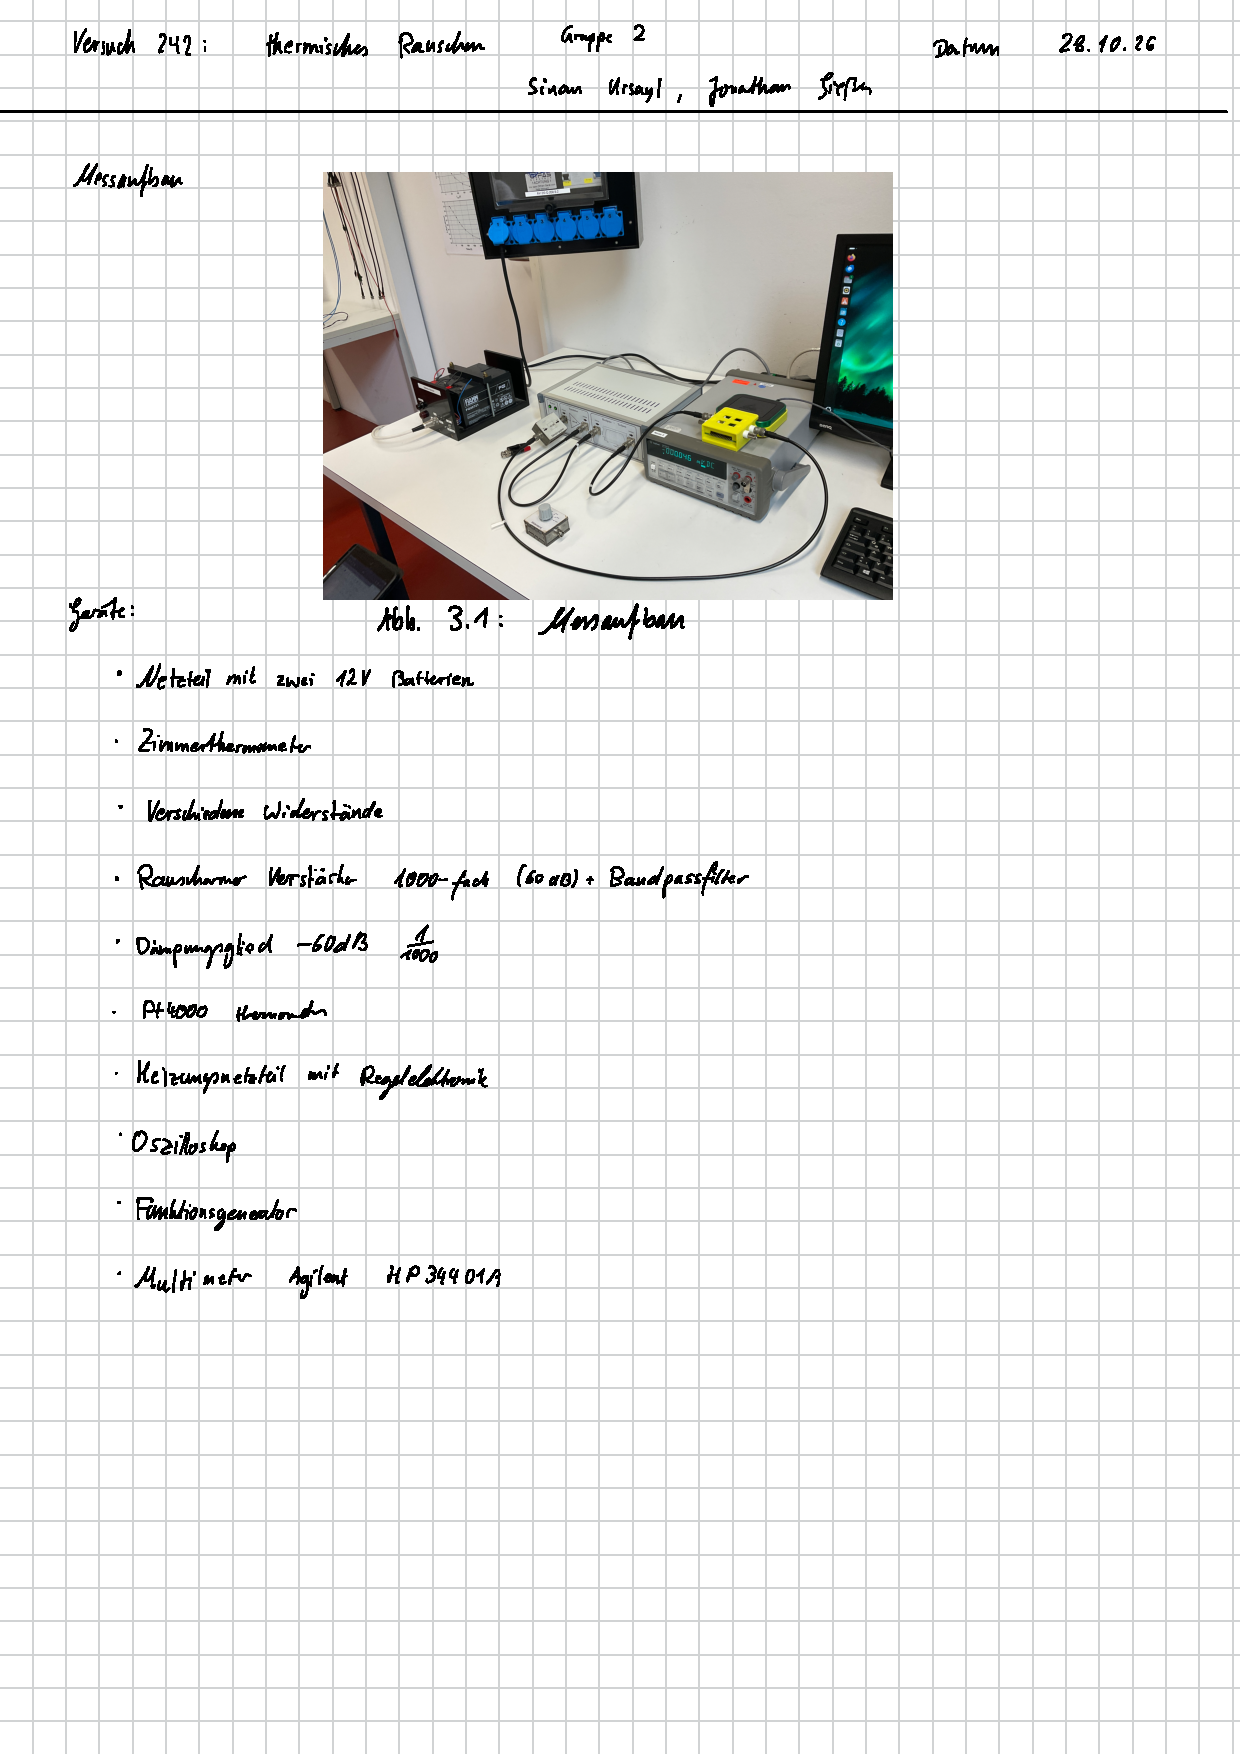
\includepdf[
    pages=-,
    width=\textwidth,
    height=0.92\textheight,
    keepaspectratio,
    pagecommand={\thispagestyle{scrheadings}},
    pagecommand*={\thispagestyle{scrheadings}\subsection{Versuchsaufbau und Aufgaben}}
]{../Messprotokoll 243.pdf}

\section{Auswertung}

\subsection{Aufgabe 1: Graphische Darstellung der Messdaten}




\clearpage

\listoffigures


\listoftables

\begin{thebibliography}{5}
    \bibitem{PAPskript} Dr. J.Wagner, \emph{Physikalisches Anfängerpraktikum IIb}, Stand 10/2026
    \bibitem{ilberg1988physikalisches} W. Ilberg, M. Krötzsch, \emph{Physikalisches Praktikum für Anfänger}, BSB B. G. Teubner Verlagsgesellschaft, Leipzig (1985).
\end{thebibliography}




\begin{comment}

\begin{table}[H]
    \centering
    \caption{Mess- und Geräteparameter für die exemplarische Berechnung (Messung 28).}
    \label{tab:parameter_messung_28}
    \begin{tabular}{ll}
        \toprule
        \textbf{Größe} & \textbf{Wert} \\
        \midrule
        Fallstrecke & $s_1 = 10\,\text{Skt} = 5.00 \cdot 10^{-4}\,\text{m}$ \\
        \bottomrule
    \end{tabular}
\end{table}
\end{comment}


\end{document}